\title{A 1.461-Approximation to Graph-TSP}
\author{
        Justin Holmgren\\               
            \and
        Lin Fei\\
}
\date{\today}

\documentclass[12pt]{article}

\usepackage{lgrind}

\usepackage[pdftex]{graphicx}
\usepackage{fancyhdr}
\usepackage{amsmath}
\usepackage{amssymb}
\usepackage{mathrsfs}

\begin{document}
\maketitle

\begin{abstract}
This reading project is based on a recent paper by Tobias Momke and Ola Svensson titled: \emph{Approximating Graphic TSP by Matching [1]}.
\end{abstract}


\section{Introduction}
The Travelling Salesman Problem (TSP) is perhaps one of the most well-known NP-Complete problems. There are many variants of the problem, to avoid ambiguity we will make the following definition:

{\bf General TSP}: Let $G = (V,E)$ be a complete graph on the set of vertices $V$. Further, assume that there exists a non-zero weight function $w$ that assigns weight to every edge. The TSP problem asks us to find a Hamiltonian cycle in $V$ of minimal weight that visits each node exactly once.

A particular variant of the general TSP specifies that the weight function $w$ satisfies the triangle inequality, that is: $w(x,y)+w(y,z) \leq w(x,z)$. This is referred to as the {\bf metric-TSP}.

A lot of work has been done to study metric-TSP. It has been shown that metric-TSP is in the class APX-hard. This implies that it is impossible to devise a Polynomial Time Approximation Scheme (PTAS) for it unless P=NP. Therefore we cannot arbitrarily approximate metric-TSP. Indeed, it is shown that it is NP-hard to approximate metric-TSP with a ratio better than 220/219 [2].

For more than 30 years, the best known approximation algorithm for metric-TSP is the Christofides [3] algorithm, which achieves an approximation ratio of 3/2.

A linear programming relaxation technique known as the Held-Karp relaxation [4] was instrumental in understanding the bounds on the approximation of metric-TSP. Like many other LP relaxation problems we learned in 6.854, it first solves the LP for continuous values of the variables, then attempts to give only integer solutions which corresponds to an actual choice of a path in the TSP. Thus, it is very important for us to understand the upper and lower bounds of the integrality gap. To this end, the best lower bound is 4/3 and is conjectured to be tight, whereas the best upper bound is obtained via Christofide's algorithm, which is 3/2.

This is where things currently stand for the metric-TSP problem, however, many interesting results have since been found for a particular kind of metric-TSP, and the upper bound have been improved. A special type of metric-TSP is referred to as graph-TSP, where we have some underlying undirected graph G with vertices V, and the weight function $w$ between two points is equal to the length of the shortest path between these two points. Note that the edges are unweighted, and ``shortest'' simply means the least *number* of edges.

Many believe graph-TSP captures the ``hardness'' of metric-TSP since it is APX-hard with a lower bound 4/3 as given by the Held-Karp relaxation. This is to be contrasted with other special cases of metric-TSP such as the Euclidean-TSP (where distances between vertices are the Euclidean distances between them), which is shown to admit a PTAS.

Recently, Gharan et al. [5] showed that graph-TSP can be approximated with a ratio strictly better than 1.5 by $\epsilon$, where $\epsilon$ is on the order of $10^{-12}$. In this paper by Momke and Svensson, the ratio is further improved to 1.461.

\section{Christofides Algorithm}

The big idea in all three of these approximation algorithms: Christofides, 3/2-$\epsilon$ and 1.461 are somewhat similar, therefore it helps to start building intuition from the simplest - Christofides. The reader should feel free to skip this section.

Christofides algorithm can be used to solve any metric-TSP (not just graph-TSP). Again, let $G=(V,E)$ be a complete graph, and let the weight function be $w$ which satisfies the triangle inequality. Christofides algorithm operates as follows:

1. Compute the minimum spanning tree $T$ of $G$.

2. Let $O$ denote the set of vertices in $T$ with odd degree. We find a minimum weight perfect matching $M$ in the complete graph over the vertices in $O$.

3. Combine the edges of $T$ and $M$ to form a multigraph $H$. (A multi-graph is just a graph that can have more than one edges between the same pair of nodes).

4. Since $M$ matches up all the odd degree nodes in $T$, $H=M\cup T$ now has only even-degree vertices, hence it is an Eulerian circuit.

5. Traverse the circuit found in the previous step and skipping visited nodes via shortcutting to make it Hamiltonian.

We will show that the above algorithm gives a 3/2-approximation.

Let $A$ denote the edge set of the optimal solution of TSP on $G$. and let $w(S)$ denote the total weight of a set $S \in E$ of edges.

{\bf Claim 1:} $w(T)\leq w(A)$.

This is true because A spans all the vertices $V$, and therefore it must contain some spanning tree, which will have a bigger weight than the MST $T$.

{\bf Claim 2:} $w(M) \leq w(A)/2$.

This is slightly less obvious. Recall $O$ is the set of vertices in $T$ with an odd degree. Suppose we want to find an optimal solution of TSP for the complete graph over vertices from $O$ only (ie, only need to make sure we visit every node in $O$), let's call the set of edges in this TSP solution $B$. Clearly $w(B)\leq w(A)$ because the tour with edge set $A$ visits more nodes, and since the weights satisfy the triangle inequality, you can never save distance by visiting more points.

Now, we show that $M$, the minimum weight perfect matching over $O$ has weight at most $w(B)/2$ which is in turn less than $w(A)/2$. First, notice that there must be an even number of vertices in $O$, and since $G$ is complete, a perfect matching exists. In particular, if we list the edges in $B$ in order: $e_1$,$e_2$,$\ldots$,$e_{2k}$, we get an Eulerian path, and we can easily see that both $e_1$,$e_3$,$\ldots$,$e_{2k-1}$ and $e_2$,$e_4$,$\ldots$,$e_{2k}$ are perfect matchings. Since their combined weight is $w(B)$, one of these perfect matchings will have at most $w(B)/2$. Hence, $M$ being the minimum weight perfect matching over $O$ will have at most $w(B)/2 \leq w(A)/2$, which proves the claim.

Combining claims 1 and 2, the total weight of the multigraph $H$ is at most $w(T)+w(M) \leq \frac{3}{2}w(A)$. This can only decrease when we take shortcuts in step 5. Thus, this algorithm yields a 3/2-approximation.

\section{Roadmap}

First let's define a few terms which will be used in this paper.

{\bf Definition:} A graph is 2-vertex-connected (2VC) if the removal of any single vertex does not disconnect the graph.

{\bf Definition:} A graph is 2-edge-connected (2EC) if the removal of any single edge does not disconnect the graph. Note that a 2VC graph is automatically 2EC.

{\bf Definition:} A graph is cubic if every node has degree exactly 3. In particular, a cubic 2-edge-connected graph is a graph that is both cubic and 2EC.

The structure and proof of the 1.461-approximative algorithm is fairly involved. At many points, we will have to assert certain theorem without proof and invite the reader to read the cited papers.

To help guide the reader through the proof, we list out the main lemmas and theorems and show their dependency graphically.

The major intermediate steps and their informal, high level descriptions are listed below:

{\bf Lemma 1:} Shows that to prove any r-approximation exist, it suffices to show that r-approximate exists for its 2VC subgraphs. Thus, we can restrict our attention entirely on 2VC graphs.

{\bf Lemma 2:} For any cubic 2EC graph, we can find a distribution of perfect matching such that each edge is included with probability exactly 1/3.

{\bf Definition 3:} We define a ``removable pairing''. Its precise definition will be clear later, for now, it can be regarded heuristically as a set of edges that can be removed to reduce the cost of the tour, while preserving the property that the path is Eulerian.

We show that we can turn any 2VC graph into a cubic graph by introducing a gadget for each node depending on its degree, we can then use lemma 2 to prove the following result:

{\bf Lemma 4:} For any 2VC graph $G$ with a removable pairing, it is possible to find a distribution over some subsets of the edges in $G$ that satisfies a set of properties which allows it to be turned into an Eulerian tour.

Using this, we can calculate the upper bound on the number of edges in the Eulerian tour in terms of the number of edges and the size of the removable pairing:

{\bf Theorem 5:} For any 2VC graph $G$ with removable pairing $(R,P)$, there exists a polynomial time algorithm that returns a spanning Eulerian multigraph with number of edges at most: $\frac{4}{3}|E|-\frac{2}{3}|R|$.

We still don't know what $\frac{4}{3}|E|-\frac{2}{3}|R|$ is, but as we will show we can transform this problem into a minimum-cost cirulation problem.

{\bf Lemma 6:} We can transform the above problem to a minimum-cost circulation problem where finding the upper bound of the number of edges in the original Eulerian multigraph is equivalent to finding the minimum-cost circulation.

We then break the circulation into two parts, and bound the cost of the two parts with {\bf Lemma 7} and {\bf Lemma 8}. Thus, we have bound the number of edges in the Eulerian multigraph, which is in turn an upperbound on the total cost of the graph-TSP. To bound the costs, it is necessary to invoke the Held-Karp relaxation.

As it turns out, the bound is dependent on $n$, the number of nodes in the original graph. Our algorithm gives a better bound $(<1.5)$ for small $n$, but asymptotes to 1.5 for large $n$. Meanwhile, Christofides gives a better bound $(<1.5)$ for larger $n$, but when $n$ is small the best upperbound is 1.5. Hence we can combine the two algorithms and claim a bound that is better than 1.5 for all $n$, that bound turns out to be 1.461.

The Roadmap of the proof is illustrated in figure 1. It is not meant to be understood upon first inspection, rather, the reader should treat it as a map so as to not get lost in the subsequent sections.

\begin{figure}[t]
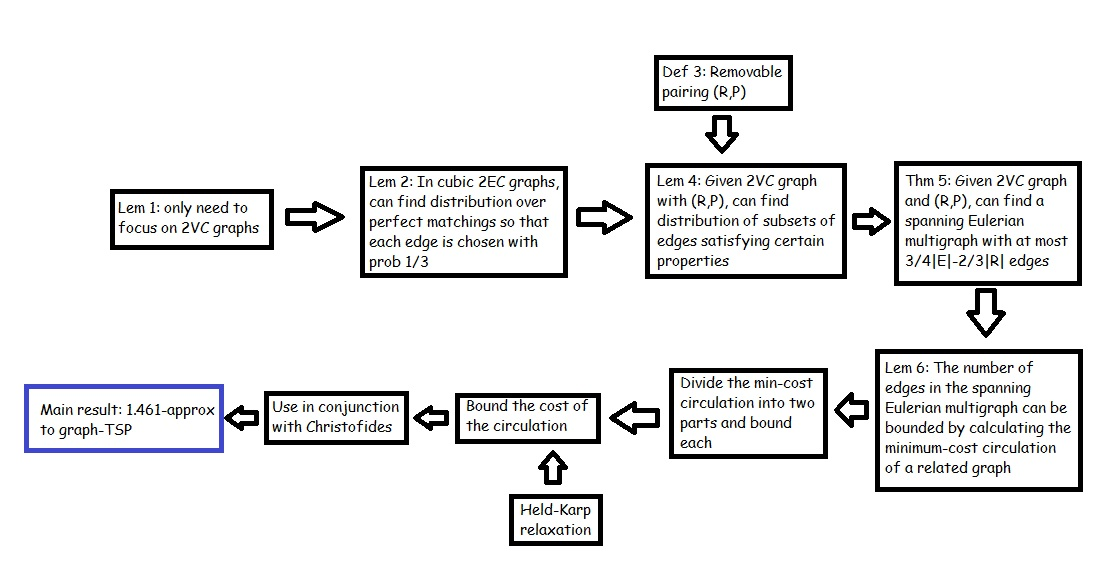
\includegraphics[width=14cm]{chart.jpg}
\caption{Roadmap of proof}
\end{figure}


\section{Held-Karp Relaxation}
We can apply LP relaxation and convert the optimal tour of a TSP into an equivalent LP. This is known as the Held-Karp relaxation. The variables are $x_{\{u,v\}}$ corresponding to each edge. Intuitively, $x_e=1$ if it is in the optimal tour and $0$ otherwise. For a general TSP problem, let $G=(V,E)$ be the complete graph on the set of vertices, and let $w_{\{u,v\}}$ be the distance between $u$ and $v$. Then, the following LP is used to find the optimal tour:

Minimize: $\Sigma_{e\in E}c_e x_e$

subject to:

$x(\delta(v))=2$ for $v\in V$,

$x(\delta(S)) \geq 2$ for $\emptyset \not= S \subset V$, and

$x \geq 0$

Where $\delta(S)$ denotes the set of edges crossing the cut $(S,\bar{S})$, and $x(F)=\Sigma_{e\in F} x_e$ for any $F \subseteq E$.

Heuristically, the equality constraint ensures that the cross across every vertex and its complement is 2, meaning that it is visited exactly once. The inequality ensures that there are at least 2 edges connecting every set $S$ and its complement, this implies that S and its complement are connected, thus this ensures the connectedness of the graph, meaning that every node is visited by a single tour.

Notice that if we let $S = v$ in the inequality constraint, we obtain $x(\delta(v)) \geq 2$ which is looser than the equality constraint ($\geq 2$ instead of $= 2$). However, Goemans and Bertsimas [6] proved that for metric distances, the looser inequality constraints do not change the optimal value of the LP. Also, for graph-TSP, the distances between each pair of vertices in the complete graph is equal to the number of edges in the shortest paths connecting them in the original graph, making $c_e = 1$. Hence, we can formulate the Held-Karp relaxation for graph-TSP as:

Minimize: $\Sigma_{e \in E} x_e$

subject to:

$x(\delta(S)) \geq 2$ for $\emptyset \not= S \subset V$, and

$x \geq 0$

We will refer to this linear program as $LP(G)$, and its optimal solution as $OPT_{LP}(G)$.

We can make an observation that allows us to concentrate the graph-TSP problem for graphs which are 2-vertex-connected. Suppose the graph is not 2-vertex-connected, suppose after removing vertex $v$ the graph will decompose into $G_1$, $G_2$, $\ldots$, $G_l$. We can then recursively solve the graph-TSP problem on the subgraphs: $G_1 \cup {v}$, $G_2 \cup {v}$, etc. The union of the solutions for the subproblems can then be combined to give a solution for the whole graph. This observation is summarized in the following lemma which we will state without proof: (for a complete proof, see [1])

{\bf Lemma 1:} Suppose $G$ is a connected graph, and $G_1$,$G_2$,$\ldots$ are 2-vertex-connected subgraphs of $G$. Suppose an $r$-approximate algorithm exists for each subgraph $G_i$ (with respect to $OPT_{LP}(G_i)$), then there is an $r$-approximate algorithm on $G$ (with respect to $OPT_{LP}(G)$).

\section{A Useful Lemma for Matchings}

Recall that finding a matching is crucial in Christofide's algorithm, so before proceeding further, we need to mention a result about matchings which will become useful later in our algorithm.

Consider a linear program whose feasible region is suppose to describe perfect matchings. It has variables $x_e$ for every $e \in E$. Intuitively, $x_e = 1$ if $e$ is in the matching, and 0 otherwise. Consider the following constraints:

$x(\delta(v)) = 1$ for $v \in V$,

$x(\delta(S))\geq 1$ for $S \subseteq V$ with $|S|$ odd, and

$x \geq 0$

To gain some intuition into why the feasible regions of the above linear program finds perfect matchings, let's suppose $x_e$ can only take on integral values 0 or 1. Then, the equality constraint ensures that every vertex $v$ has exactly one edge incident from it. This ensure that the edge set chosen is a matching.

Then, to motivate why it is a perfect matching, we look at a set $S$ with an odd number of vertices, we know at least one of them is matched with some other node in $\bar{S}$, hence the second inequality constraint.

Edmonds [7] showed that the above set of constraints define what is called the perfect matching polytope, where all extreme points of the polytope are integral and correspond to perfect matchings. This result is true for a general graph.

For a special type of graph that are cubic and 2-edge connected (i.e. every node has degree 3, and the graph is still connected after removing any edge), Naddef and Pulleyblank [8] proved that $x_e = 1/3$ for all $e \in E$ is inside the feasible region.

Now if we consider the objective function $\Sigma_{e\in E}x_e$, by properties of extreme points, we know that at least one of the extreme points will have a better objective value than the $x_e = 1/3$ feasible point in the interior of the polytope. This implies that in any cubic 2-edge-connected graphs, there always exists a perfect matching of weight at least 1/3 of the total weight of edges.

Now we invoke Caratheodory's theorem (see Thm 6.5.11 in [9]) which says that we can, in polynomial time, decompose a feasible solution in the perfect matching polytope into a linear combination of polynomially many perfect matchings. Suppose we regard the coefficients of this linear combination $\lambda_1, \lambda_2,\ldots$ as probabilities, and we choose a particular perfect matching $M_i$ with probability $\lambda_i$, and combining with the above result by Naddef and Pulleyblank, we can assert that the probability of any edge being included in a perfect matching is exactly 1/3. We summarize this in the following lemma:

{\bf Lemma 2:} Given any cubic, 2-edge-connected graph $G$, we can, in polynomial time, find a probability distribution over polynomially many perfect matchings such that the probability of any edge being chosen as part of a perfect matching is 1/3.

Notice that a 2-vertex-connected graph is automatically 2-edge-connected, unless it is the graph with 2 vertices and 2 edges connecting between them. Therefore, we can apply lemma 2 to cubic 2-vertex-connected graphs. Recall from lemma 1 that we can focus our attention to 2-vertex connected graphs, though in general they may not be cubic.

\section{Main Insight of the Algorithm: Removable Pairs}

With the preliminaries out of the way, we are now ready to describe the main features of this 1.461-approximate algorithm to graph-TSP.

Recall in Christofides algorithm, we first find the MST $T$ of $G$, then ``fix up'' the odd degree nodes with a min weight matching $M$ to get an Eulerian multigraph $H = T\cup M$. 

Other algorithms for TSP employs a similar structure, except that instead of finding the minimum spanning tree, they use a minimum cost spanning 2-vertex-connected subgraph. But the use of matching is similar. Typically they find the minimum matching and add it to the 2-vertex-connected subgraph to arrive at an Eulerian multigraph. The main difference of this paper by Momke and Svensson is that instead of just adding edges from the matching $M$ to the 2-vertex-connected subgraph, they showed that certain edges in $M$ can instead be taken out of the 2-vertex-connected subgraph to yield a lower cost, while still maintaining the property that the resulting graph is Eulerian.

This prompts us to use the following definition, which may seem ad hoc now, but will become more clear later on.

{\bf Definition 3: (removable pairing of edges)}
Given a 2-vertex-connected graph $G$, we call a tuple ($R$,$P$) consisting of a subset $R$ of removable edges and a subset $P \subseteq R \times R$ of pairs of edges a removable pairing if:

1. an edge is in at most one pair;

2. the edges in a pair are incident to a common vertex of degree at least 3;

3. any graph obtained by deleting removable edges so that at most one edge in each pair is deleted stays connected.

Now we are ready to prove the following lemma:

{\bf Lemma 4:} Given a 2-vertex-connected graph $G=(V,E)$ with a removable pairing ($R$,$P$) defined above, we can, in polynomial time, find a probability distribution over polynomially many subsets of edges such that a random subset $M$ form this distribution satisfies:

1. each edge is in $M$ with probability 1/3;

2. at most one edge in each pair is in $M$; and

3. each vertex has an even degree in the multigraph with edge set $E \cup M$.

{\bf Proof}. We would like to transform $G$ into $G'$ which is a cubic 2-edge-connected graph, so that we can apply lemma 2. To do this, we transform every node that does not have a degree equal to 3. We will create a gadget for each type of node with degree not equal to 3.

Since $G$ is 2-vertex-connected, clearly there can be no node of degree one, otherwise, we can just remove its only neighbor and it would be disconnected.

1. For a vertex of degree 2, we replace that vertex with 4 new nodes as shown in the figure

2. for a vertex with degree $d(v)>3$, we replace that vertex with a tree of $\lfloor \frac{d(v)}{2} \rfloor$ nodes. We ensure that every node inside the tree has degree 3. At each leaf node, we connect it to two edges originally in $G$ such that if two edges $(e_1,e_2)\in P$, we make sure they get mapped to the same leaf node. When $d(v)$ is odd, there will be one extra edge remaining, we can fix this by connecting it to the root of the tree and making sure the root only has 2 children. Please see the graph for a few examples of this construction. Note that if we want to increase the degree by 2, we just simply split a leaf node and make it into two new leaf nodes while still satisfying the requirement that all nodes have degree 3.

\begin{figure}[t]
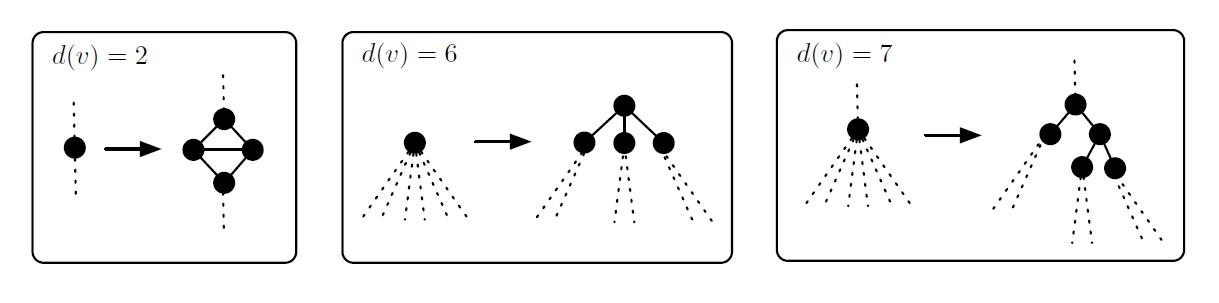
\includegraphics[width=14cm]{gadget.jpg}
\caption{Examples of the used gadgets to obtain a cubic graph}
\end{figure}

Using these gadgets, we have turned $G$ into $G'$, which is 2-vertex-connected and cubic. This means we can apply lemma 2 to obtain a random perfect matching $M'$. We know each edge in $G'$ will be included in $M'$ with probability 1/3. Restricting the set $M'$ to the graph $G$ in the obvious way, we obtain $M$. Obviously, every edge in $G$ will be in $M$ with probability 1/3, satisfying the first requirement.

For the second requirement, suppose that both edges in a pair are in $M$. By the definition of a pair, they must be connected to a node of degree at least 3. That means, by the way we constructed the gadgets, the two edges in the pair will be connected to the same node in $G'$, which means that they cannot both be in the matching $M'$. Hence, at mot one edge in each pair is in $M$.

For the third requirement, simply note that we are compressing the graph $G'$ to get to $G$. $M'\cup E'$ is an Eulerian tour of $G'$, which means that its nodes all have even degrees. The compression of a edge set with even degrees will again be an edge set of even degrees. Therefore $M\cup E$ is a spanning Eulerian tour. Thus completing the proof.

We now use lemma 4 to prove a theorem which will be central to the rest of our analysis.

{\bf Theorem 5:} Given a 2-vertex-connected graph $G = (V,E)$ with a removable pairing (R, P), there is a polynomial time algorithm that returns a spanning Eulerian multigraph in $G$ with at most $\frac{4}{3}|E| - \frac{2}{3}|R|$ edges.

{\bf Proof:}
We begin by picking a random subset $M \subseteq E$ of edges that satisfies the properties of lemma 4. Let $M_R$ be the set of those edges of $M$ that are removable and let $\bar{M_R}$ be the set of the remaining edges of $M$.

Consider the multigraph $H = E\cup \bar{M_R} - M_R$, i.e. instead of adding all the edges in $M$ into $E$, we remove the ones in the removable set. Since property 3 of the lemma ensures that $E\cup M$ has all even degrees, and add or removing an edge changes the parity of nodes in the same way, we must also have that $H$ has all even degrees. Further, since $(R,P)$ is a removable pairing, property 2 of lemma 4 ensures that $H$ is connected. Therefore we can conclude that $H$ is an Eulerian graph, i.e a solution to the graph-TSP problem.

Now we calculate the expected number of edges in $H$.
\begin{equation}
\mathcal{E}[|E|+|\bar{M_R}|-|M_R|]
\end{equation}

Using Linearity of expectation, this can be evaluated to be:

\begin{equation}
|E| + \frac{1}{3}(|E|-|R|)-\frac{1}{3}|R| = \frac{4}{3}|E|-\frac{2}{3}|R|
\end{equation}

Notice that in lemma 4, there are only a polynomial number of perfect matchings in the distribution, therefore we can simply check through all of them and take the one with the least number of edges, this gets rid of the randomization in the algorithm, and clearly, the choice with the least number of edges will have at most $\frac{4}{3}|E|-\frac{2}{3}|R|$ edges. This concludes the proof.


\section{Relating the Number of Edges to a Minimum-Cost Circulation}

In Theorem 5, we showed that given a 2-vertex connected graph $G$ with a
removable pairing $(R, P)$, we can find a Hamiltonian cycle with cost at most
$\dfrac{4}{3} \cdot |E| - \dfrac{2}{3} \cdot |R|$.  This bound is as yet
unsatisfactory, because $|E|$ may be extremely large and $|R|$ may be small.
What we'd like to do is find a \emph{small} spanning 2-vertex-connected
subgraph $G'$ of $G$ with a large removable pairing $(R, P)$ on $G'$, such that
Theorem 5's bound is tighter.  We will show that we can find such a subgraph
$G'$ and a removable pairing $(R,P)$ by solving a certain min-cost circulation
problem.

We start with a spanning tree $T$ of $G$ which is obtained by a DFS, and use
$T$ to classify the edges of $G$ as directed edges which are either {\bf tree
edges}, which are in $T$ and directed towards $T$'s leaves, and {\bf back
edges}, which are directed towards the root.  Notably, there are no cross edges.

We extend $G$ to obtain a min-cost circulation problem $C(G, T)$ with integer
edge flow lower bounds, and integer costs and weights.  By Hoffman's circulation
theorem (see Corollary 12.2a in [10]), there exists an integer solution. Every tree edge has a
flow lower bound of $1$, and $G'$ is the set of all edges in $G$ which
correspond to positive-flow edges in $C(G,T)$, so $G'$ will clearly span $G$.
No other edge has a flow lower bound.  

We would like to distinguish back-edges that come from different sub-trees to
make sure that the graph stays connected when edges are removed, so we introduce
some new nodes.  For every node $v$ besides the root, we introduce new nodes
$v_1, \ldots, v_l$ between $v$ and each of its children.  For such $v$ , we
redirect all of $v$'s incoming back edges to the child $v_i$ which lies between
$v$ and the other endpoint of the back edge.  We will call these vertices
\emph{in-vertices}, and denote the set of in-vertices by $\mathcal{I}$.

All tree edges have cost $0$, and all back edges have cost $1$, with one
caveat.  Any given node can accept one unit of back-flow for $0$ cost.  This
can be accomplished with standard min-cost circulation algorithms via an
intermediate node with an edge of cost $0$, capacity $1$, and an edge of cost
$1$, infinite capacity.  

Let $B(v)$ denote the set of back edges ending at $v$.  Let $f(S)$ denote the
amount of flow along the set of edges $S$.

The cost $c(C)$ is
\[
\sum_{v \in \mathcal{I}} \max ( f(B(v)) - 1, 0)
\]

Now we give what the removable pairing $(R, P)$ is, but we will postpone
actually showing that it is a removable pairing.  

We will define $R$ and $P$ on $C(G, T)$, but they reduce to a removable pairing
on $G'$ quite easily.  $P$ consists of all pairs of zero-cost back edges and
tree edges which meet at an in-vertex with degree at least three.  Note that the
restriction of having degree at least three will only ever exclude the root
node, because every other in-vertex has an in-bound tree edge, and out-bound
tree edge, and we have already hypothesized that it has an in-bound back edge.
Since each in-vertex only has one inbound zero-cost back edge, all zero-cost
back edges except possibly one to the root are included in $P$.

$R$ is $P$ union all other back edges.  So $R - P$ is the set of all positive-cost back
edges, and possibly one zero-cost back edge to the root.  This implies that $|R|
- 2|P| \le c(C) + 1$.  Furthermore, the number of edges in $G'$ is the tree
  edges + the positive-flow back edges, which is at most $ (n - 1) + |R| - |P|$
(we need to count the zero-cost edges).

This means, once we show that $(R, P)$ meets the criteria for being a removable
pairing, Theorem 5 will imply that $G'$ has a spanning Eulerian multigraph
with at most $\dfrac{4}{3}((n-1) + |R| - |P|) - \dfrac{2}{3} |R| = \dfrac{4}{3}n
+ \dfrac{2}{3}(|R| - 2|P|) \le \dfrac{4}{3} n + \dfrac{2}{3} c(C^*) -
\dfrac{2}{3}$ edges. 

We now need to show that $(R, P)$ is a removable pairing.

First, an edge is in at most one pair of $P$.  $P$ was defined as all pairs of
zero-cost back edges and tree edges which meet at an in-vertex with degree at
leaset three.  Zero-cost back edges and tree edges are uniquely defined by the
in-vertex that they touch, so it is clear that all these pairs will be disjoint
from each other.  When we reduce to $G'$ from $C(G, T)$, neither of these two
edges are part of the 

Second, the edges in a pair are incident to a common vertex of degree at least
$3$.  This is by construction of $P$.  When we reduce to $G'$ from $C(G,T)$,  the
degree of the edges' common node will still be at least $3$, because they will
still have an in-bound tree edge.

Finally, we need to show that if we remove edges in $R$ such that we remove no
two edges from the same pair in $P$, the graph stays connected.  To prove this,
we use induction on the height of a subtree.  For leaves, of course removing
edges will not disconnect a leaf vertex from itself.  For a subtree of height
$h$, by induction each of its sub-trees remains connected, and we just need to
show that the root $v$ of this subtree remains connected to each subtree.  Suppose
that the edge between $v$ and one of its children has been deleted.  Since this
is a tree edge, the other element in its pair must have been a back-edge from
this child's subtree to $v$, which cannot have been deleted, so $v$ remains
connected.

% TODO: Examples of transformations go here

\section{Bounding the Circulation}

Recall that for a graph $G$, $LP(G)$ refers to the Held-Karp linear program for
$G$, in which variables correspond to fractional edge inclusion, and the
fractional magnitude of each non-trivial cut is at least 2.  It is a known fact
% TODO cite
(we will not prove it) that an extreme point of $LP(G)$ has at most $2n-1$
non-zero variables.  We call this set of non-zero variables the {\bf support} of
the extreme point, and we call the corresponding set of edges $E'$.  We use
$OPT_{LP}(G))$ primarily as a lower bound on the optimum path in order to prove
approximation ratios.

That is, we say we have an $r$-approximation relative to $LP(G)$ if our
solution's  magnitude is within a factor of $r$ of $OPT_{LP}(G)$.  An
$r$-approximation relative to $LP(G)$ is also just an $r$-approximation, because
$OPT_{LP}(G)$ is less than or equal to the optimal integral solution.

Now, consider the graph $G = (V, E')$.  $OPT_{LP}(G') = OPT_{LP}(G)$ because by
construction, $E'$ corresponds to a small set of edge variables which are sufficient
to achieve $OPT_{LP}(G)$.  So we just need to be able to find an
$r$-approximation for graphs with $n$ vertices and at most $2n-1$ edges.

Let $x_a$ denote the value corresponding to edge $a$ in $LP(G')$.  For reasons that will
become apparent in our analysis, we choose a tree $T$ for $G'$ with a DFS from an
arbitrary node, but when we have a choice of which edge to traverse first, we
pick the edge with the highest corresponding value in $LP(G'))$.

Now to bound the minimum circulation in $C(G', T)$, we give an example
circulation with a boundable value.  Our circulation $f$ consists of two parts,
which we will call $f'$ and $f''$.  $f'$ consists of, for each back edge $e$,
sending $\min(x_e, 1)$ unit of flow along the (unique) cycle containing only $e$
and tree edges.

For this circulation to be feasible, we also need to ensure that each tree edge
has flow at least 1.  This is what $f''$ does.  Because from an in-vertex, there
is only one place for flow to go (along the outbound tree edge), it is
sufficient to consider to require only that the flow going into each in-vertex
along a tree edge is at least 1. For each tree edge $(v, w)$, where $v$ is an
out-vertex, and $w$ is a child of $v$, $f'(v,w)$ is less than 1, $f''$ sends $1
- f'(v,w)$ flow along some cycle containing $(v,w)$ and a back edge.  There must be
such a cycle, because otherwise we could show that 2-vertex-connectedness is
violated.

Now we analyze the cost of this circulation.  This is mostly algebra, but there
are a few insights for each part.

The total cost is equal to
\[
\sum_{v \in \mathcal{I}} \max(f(B(v))-1, 0)
\]
which is upper-bounded by
\[
\sum_{v \in \mathcal{I}} \max(f'(B(v))-1,0) + \sum_{v \in \mathcal{I}} f''(B(v))
\]
because for any real $x$, $y$, if $y \ge 0$, $\max \left ( x, 0 \right ) + y \ge \max
\left ( x + y, 0 \right )$.

First we will analyze the second term above.
{\bf Lemma 7:}
$sum_{v in \mathcal{I}} f''(B(v)) \le OPT_{LP}(G) - n$.

We claim that $\sum_{v in \mathcal{I}} f''(B(v)) \le OPT_{LP}(G) - n$.
Also, $\sum_{v \in \mathcal{I}} \max(f'(B(v)) - 1, 0) \le (7 - 6 \sqrt{2})n +
4(\sqrt{2} - 1)OPT_{LP}(G)$.  
Combining the two gives us that the cost of the circulation is upper-bounded by
$6(1- \sqrt{2})n + (4\sqrt{2} - 3)OPT_{LP}(G)$.

On the other hand, Christofides' algorithm can also be analyzed with an
approximation ratio in terms of $OPT_{LP}(G)$, and its approximation ratio is
$\dfrac{n + OPT_{LP}(G)/2}{OPT_{LP}(G)}$.

By solving $LP(G)$, we can pick whichever would perform better, and achieve an
approximation ratio of $\dfrac{14(\sqrt{2} - 11)}{12\sqrt{2} - 13}$, which is
about $1.461$.

\section{Bibliography}

1. Tobias Momke, Ola Svensson. Approximating Graphic TSP by Matchings. arXiv:1104.090.

\noindent
2. Christos H. Papadimitriou and Santosh Vempala. on the approximability of the traveling salesman problem. \emph{Combinatorica}, 26(1):101-120, 2006.

\noindent
3. Nicos Christofides. Worst-case analysis of a new heuristic for the travelling salesman problem. Technical Report 388, Graduate School of Industrial  Administration, Carnegie-Mellon University, 1976.

\noindent
4. Michael Held and Richard M. Karp. The travelling-salesman problem and minimum spanning trees. \emph{Operations Research}, 18:1138-1162, 1970.

\noindent
5. David Gamarnik, Moshe Lewenstein, and Maxim Sviridenko. An improved upper bound for the TSP in cubic 3-edge-connected graphs. \emph{Operations Research Letters}, 33(5): 467-474, 2005.

\noindent
6. Michel X. Goemans and Dimitris J. Bertsimas. On the parsimonious property of connectivity problems. In \emph{Proceedings of the 1st annual ACM-SIAM symposium on Discrete Algorithms (SODA 1990)}, pages 388-396, 1990.

\noindent
7. Jack Edmonds. Maximum matching and a polyhedron with 0,1 vertices. \emph {Journal of Research of the National Bureau of Standards}, 69:125-130, 1965.

\noindent
8. Denis Naddef and Wiliam R. Pulleyblank. Matchings in regular graphs. \emph{Discrete Mathematics}, 34(3):283-291, 1981.

\noindent
9. Martin Grotschel, Laszlo Lovasz, and Alexander Schrijver. \emph{Geometric Algorithms and Combinatorial Optimization}, volume 2 of \emph{Algorithms and Combinatorics}. Springer, 1988

\noindent
Alexander Schrijver. \emph{Combinatorial Optimization}. Springer, 2003.

%\bibliographystyle{abbrv}
%\bibliography{simple}




\end{document}
